\chapter{Experimental Setup}

There are some crucial components needed in order to carry out the experiment of the proposed solution. Note that in the oil cycle part of ORC, there is an already installed bypass line. This bypass line can be used to reduce the cost of implementing the proposed solution.

\begin{enumerate}
    \item First of all, a pump is needed to establish a flow in the reverse direction of the cycle.
    \item Second, a check valve is needed to ensure fluid flow only in one direction in the bypass line.
    \item Third, a 3-way valve and an actuator must be employed at the entrance of the bypass line to control the mass flow rate that will flow inside the bypass pipeline
    \item Lastly, a power source for the actuator is needed.
\end{enumerate}

\section{Concept Setup of the Proposed Solution}

\begin{figure}[H]
		\centering
		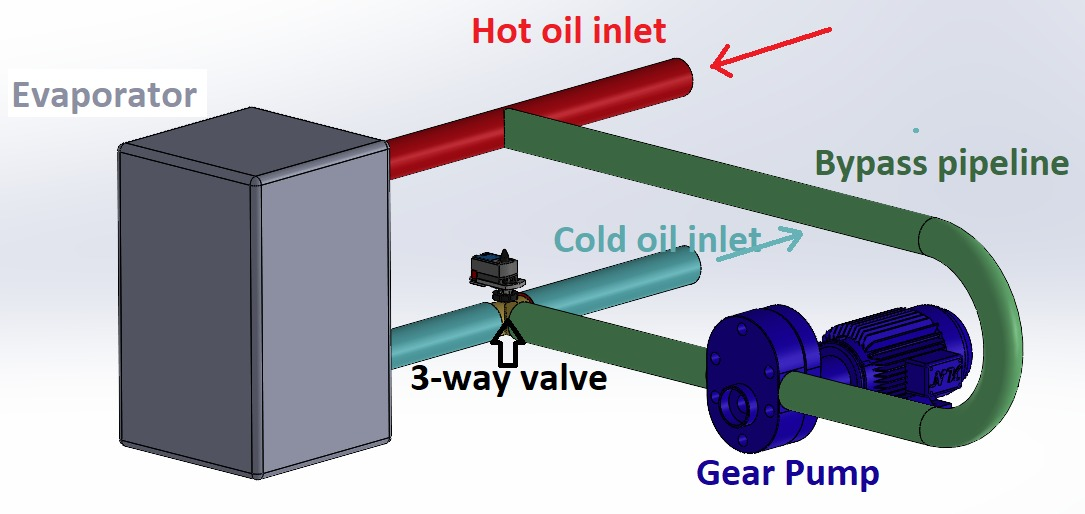
\includegraphics[width=0.8\textwidth]{images/tasarim.jpg}
		\caption[Concept Setup of the Proposed Solution]{Concept Setup of the Proposed Solution}
		\label{concept} 
\end{figure} 

The bypass pipeline connects the exit of the evaporator to the inlet of the evaporator. Since there is a height difference between the inlet and exit of the evaporator and there is a pressure loss inside the evaporator, it is not possible to constitute a flow from exit to inlet without a pump. Therefore, an appropriate pump is needed to be installed in order to employ a reverse flow. There are some crucial criteria for the pump. The pump must endure temperatures as high as $140^\circ$. Additionally, the pump must not corrode by oil. Generally, in high-temperature oil applications, gear pumps that are capable of enduring high-temperature oil are used. The head a gear pump provides is not much important since there is a small height difference between the inlet and the exit, and the pressure loss inside the evaporator is negligibly low, according to Ertugrul's thesis. A gear pump is approximately 5500 TLs.

\begin{figure}[H]
		\centering
		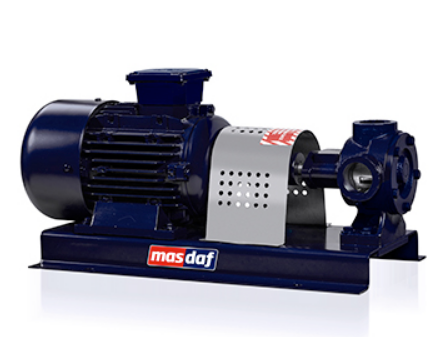
\includegraphics[width=0.5\textwidth]{images/pump.png}
		\caption[A Gear Pump]{A Gear Pump}
		\label{pump} 
\end{figure} 

Moreover, a proper check valve must be installed as well to ensure a one-direction-only flow. The same criteria are valid for the check valve: the valve must endure high-temperature oil. For this use, a disc type of check valve made up of stainless steel can be installed since it can endure high temperatures and will not corrode because of its material. This type of check valve is around 500 TLs.

\begin{figure}[H]
		\centering
		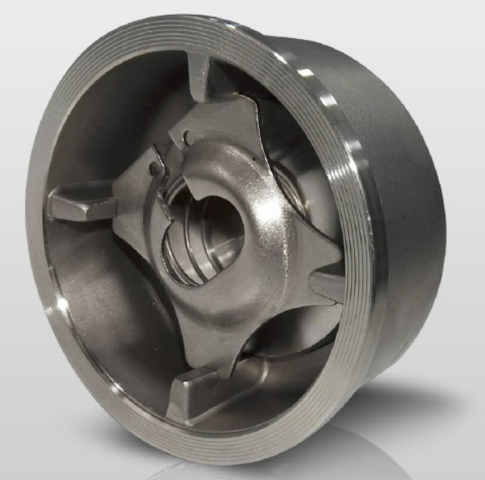
\includegraphics[width=0.3\textwidth]{images/valve_2.png}
		\caption[A Disc Check Valve]{A Disc Check Valve}
		\label{valve_2} 
\end{figure} 

Additionally, a 3-way valve will be used to establish an adjustable fluid flow direction. There are a couple of options for the type of 3-way valve, but since there is an available 3-way ball valve in the BURET lab, there is not much reason to purchase a new valve. The available 3-way ball valve is Siemens VB61.50-40 DN50 which is a brass valve with a stainless steel ball. The ball can be rotated by rotating the rectangular-shaped pin above the ball. 

\begin{figure}[H]
		\centering
		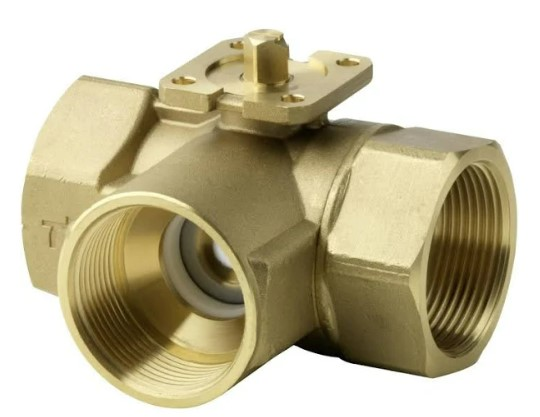
\includegraphics[width=0.3\textwidth]{images/valve.jpg}
		\caption[3-way ball valve]{3-way ball valve}
		\label{valve} 
\end{figure} 

Additionally, an actuator is needed to control the fluid flow direction by rotating the ball inside the valve. There is also an available actuator in the BURET lab, which is Siemens GLB161.9E. The actuator is coherent with the 3-way ball valve, so it can rotate the pin on the valve. Furthermore, there must be a 24V power supply for the actuator to rotate.

\begin{figure}[H]
		\centering
		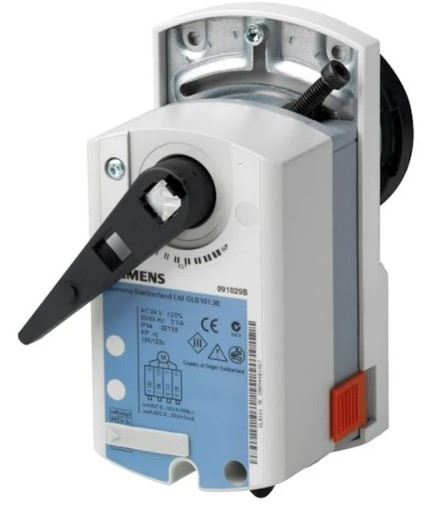
\includegraphics[width=0.3\textwidth]{images/actuator.jpeg}
		\caption[Actuator - Siemens GLB161.9E]{Actuator - Siemens GLB161.9E}
		\label{actuator} 
\end{figure} 

\par
In Table \ref{tab:components}, the components required for applying our solution method are listed with the corresponding costs.

%% TABLE
\begin{table}[h]
    \centering
    \begin{tabular}{|c|c|}
         \hline 
         \textbf{Components}    & \textbf{Cost}  \\
         \hline
         Three-way valve        &  4400 TL         \\
         Gear pump              &  5500 TL         \\
         Disc check valve       &  500  TL         \\
         Rotary actuator        &  2300 TL         \\
         \hline
         \textit{Total cost}    &  12700 TL         \\
         \hline
    \end{tabular}
    \caption{Components and costs.}
    \label{tab:components}
\end{table}

Since the bypass pipeline, 3-way ball valve, and actuator are already available, the initial cost of setting this experiment up is around 6000 TLs. Due to the cost limitations, however, a more comprehensive experiment that consists of a pump and a check valve is not done. Instead, our experimental setup will cover controlling an actuator connected to a 3-way ball valve which will control the mass flow rate in the bypass pipeline.

\section{Setup of the Experiment}

The setup of the experiment consists of three main parts, which are a 3-way ball valve, an actuator, and a power supply. There are also some cables, a resistance, and a potentiometer used. The purpose of the experiment was to establish a setup that can control the actuator's angle, which represents how much the ball valve supplies fluid to the bypass pipeline. The actuator has four cables connected to it which are the power inlet, the ground, the control, and the feedback cables. A 24V power supply is added to the setup to power the actuator. The power inlet and ground cables of the actuator are connected to this power supply.

By controlling the voltage across the control and feedback cables, the actuator can be rotated between $0^\circ$  which represents that the ball valve is closed, meaning there will be no flow to the bypass pipeline, and $90^\circ$ which represents the ball valve closed the inlet of the evaporator and fully opened the bypass pipeline. Since a closed evaporator inlet is not desired in the experiment, the actuator should never be rotated to $90^\circ$.

To control the voltage across the control and feedback cables, a simple electronic circuit must be established. The rotation of the actuator is related to the voltage difference between the feedback and control cables. If the feedback's voltage is more than the control cables, then the actuator rotates toward $90^\circ$. If the voltage across the control is more than the feedback's, then the actuator rotates toward $0^\circ$. The actuator stops when the voltage across the control and feedback cables are nearly equal to each other. The mechanism of the actuator requires that an adjustable resistance should be placed to control the voltage. Therefore, a potentiometer is placed between the control cable and the ground to establish an adjustable voltage across the control cable. Additionally, the feedback cable must be connected to a resistor before the ground. Otherwise, the voltage across the feedback 
will always be bigger than the control's voltage.

\begin{figure}[H]
		\centering
		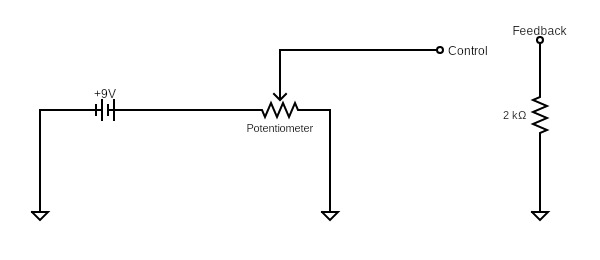
\includegraphics[width=0.7\textwidth]{images/devre.jpg}
		\caption[Circuit Diagram of the Experiment Setup]{Circuit Diagram of the Experiment Setup}
		\label{devre} 
\end{figure}


\begin{figure}[H]
    \centering
    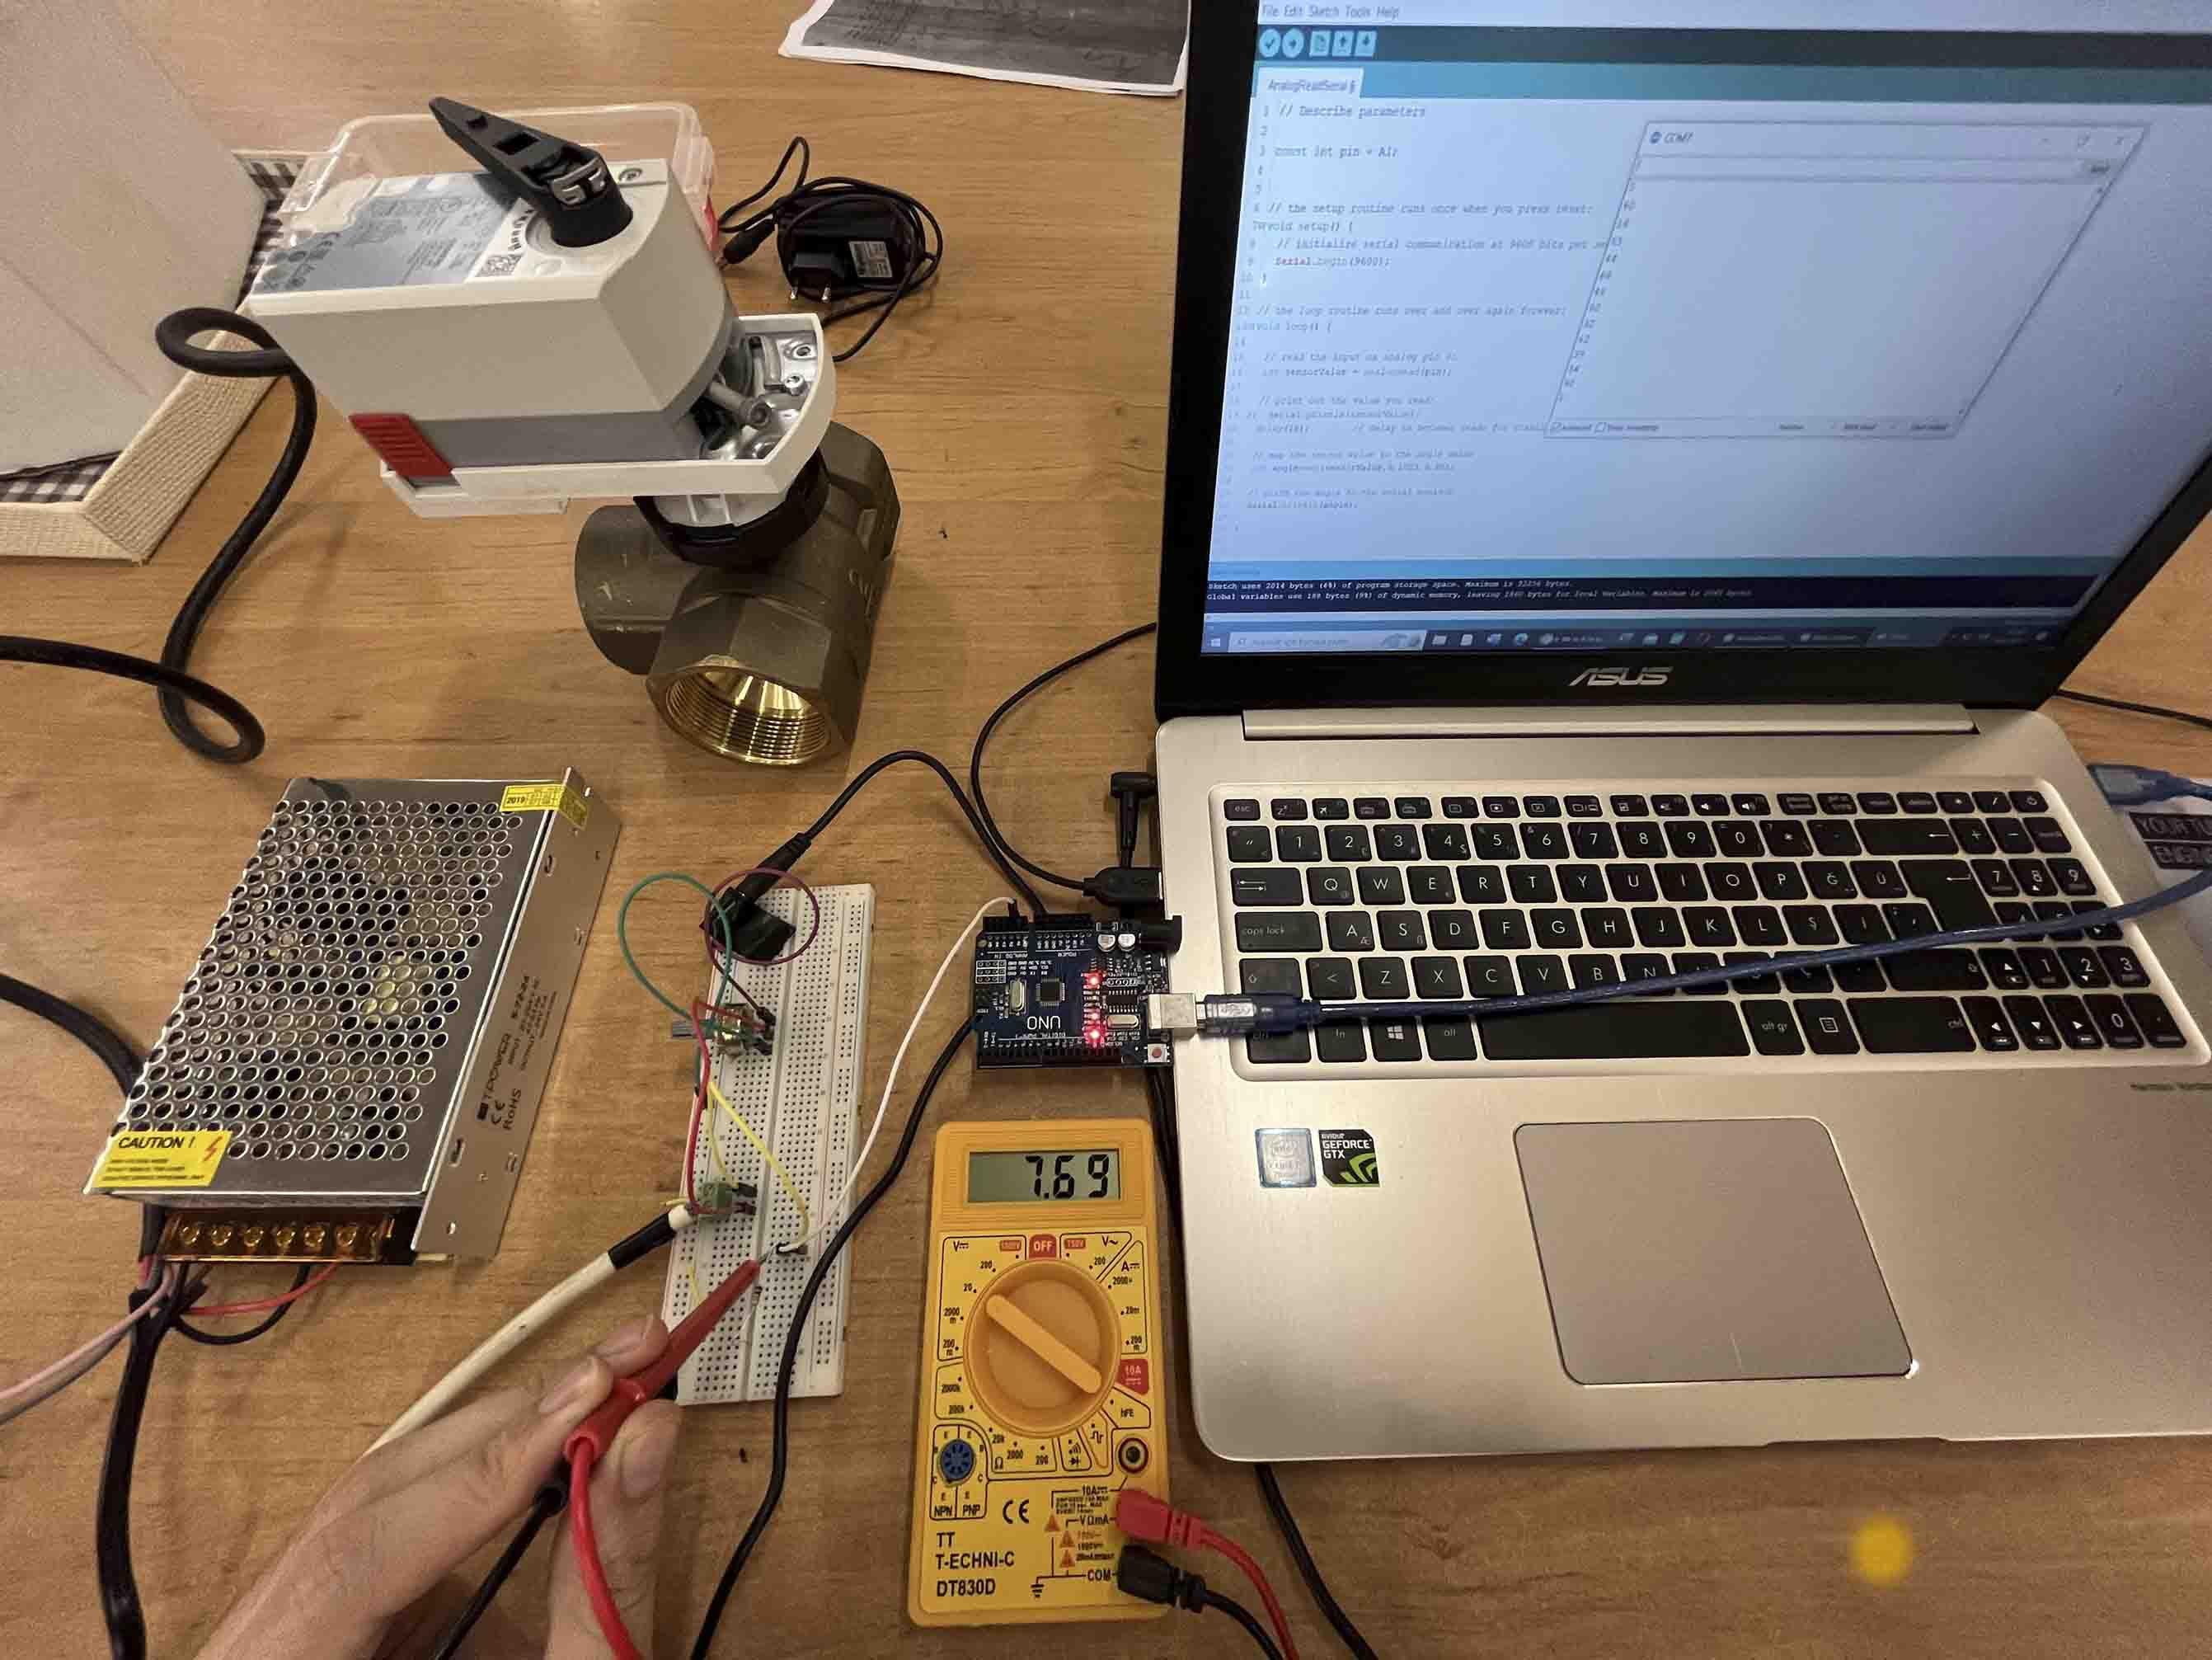
\includegraphics[width=15cm]{images/actuator.jpg}
    \caption{Actuator motor control.}
    \label{fig:actuator}
\end{figure}

\par
In case of a possible real-world implementation, the damper actuator is tested. It is connected to the three-way valve, and then the valve is opened and closed respectively. In order to do that, all connections of the actuator are made. It is connected to a 24V DC power supply, its control signal is connected to a 12V DC power supply, and its voltage is controlled by a 10k potentiometer. The feedback signal is connected to the Arduino's A1 analog input port. The incoming signal is converted to the angle and read from the serial monitor. Several positions are tested, and a video recording is completed during this process.

\par
This damper actuator control setup is shown in Figure \ref{fig:actuator}

